Для демонстрации перехода EP-LP можем рассмотрим также эксперимент по реализации одномерной системы \cite{schreiber_observation_2015}. Теперь рассматривается движение в quasi-random optical lattice созданной двумя решетками с несоизмерным шагом, но в целом всё также описывающейся гамильтонианом \eqref{9:model}.



\begin{figure}
    \centering
    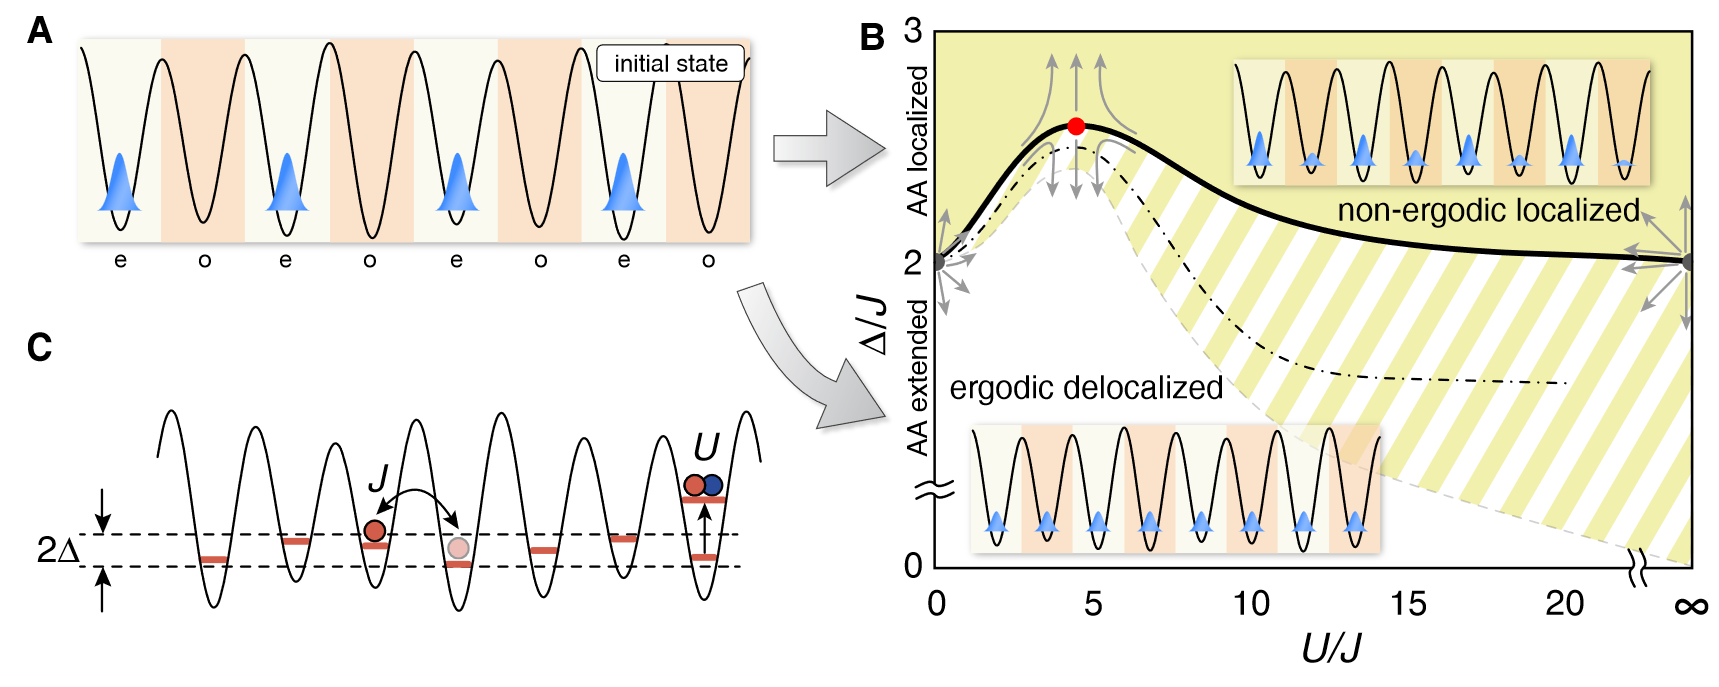
\includegraphics[width=0.7\textwidth]{imgs/1d_phases.png}
    \caption{\cite{schreiber_observation_2015} a) Initial state of the system consisting of a charge density wave, where all atoms occupy even sites only. For an interacting many-body system, the evolution of this state over time depends on whether the system is ergodic or not. b) Schematic phase diagram for the system: in the ergodic, delocalized phase (white) the initial state quickly decays, while it persists for long times in the non-ergodic, localized phase (yellow). c) Schematic showing a visual representation of the three terms in the Hamiltonian. }
    \label{fig:1Dmain}
\end{figure}




Теперь в качестве $\Omega_1$ выбраны нечётные узлы и также исследуется на сколько быстро исчезнет и до какой степени контрастность $\mathcal{I}$ заселенности чётных и нечётных узлов (fig. \ref{fig:loc1D1}). Видно, что за $t \approx 15 \tau$ наблюдаемая $\mathcal{I}$ также выходит на стационарное значение (fig. \ref{fig:loc1D1}a), где по результатм усреднения в желтой области строится зависимость $\mathcal{I}(\Delta)$ (fig. \ref{fig:loc1D1}b).

\begin{figure}
    \centering
    \addletter{45}{a}
    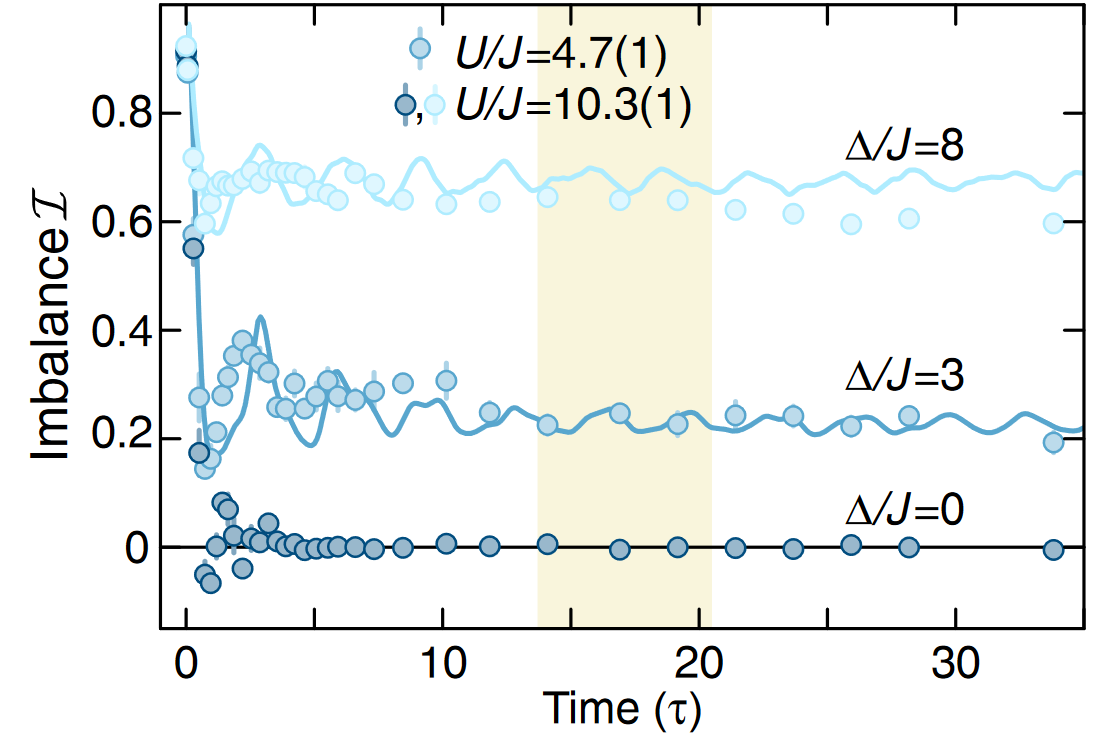
\includegraphics[align=c, width=0.35\textwidth]{imgs/MBL_exp_1.png}
    \hspace{10 mm} 
    \addletter{45}{b}
    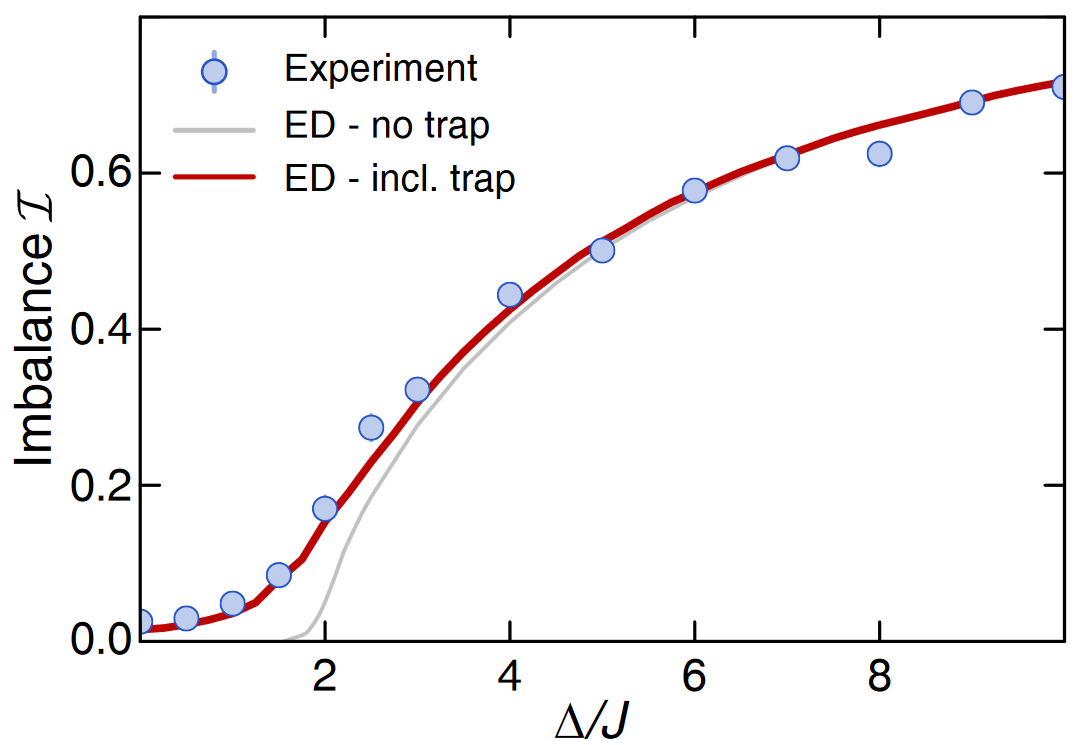
\includegraphics[align=c, width=0.35\textwidth]{imgs/MBL_exp_2.png}
    \caption{
    \cite{schreiber_observation_2015} 
    a) Time evolution of an initial charge-density wave
    . 
    b) Stationary values of the imbalance $\mathcal{I}$ as a function of disorder $\Delta$ for non-interacting atoms 
    .
    }
    \label{fig:loc1D1}
\end{figure} 





% \red{Основной вывод от этой картинки и этой статьи: есть локализация и термолизация. Взаимодействие влияет, но не столь принципиально.}}